%\documentstyle[epsf,twocolumn]{jarticle}       %LaTeX2e仕様
\documentclass[twocolumn]{jarticle}     %pLaTeX2e仕様(platex.exeの場合)
% \documentclass[onecolumn]{ujarticle}   %pLaTeX2e仕様(uplatex.exeの場合)
%%%%%%%%%%%%%%%%%%%%%%%%%%%%%%%%%%%%%%%%%%%%%%%%%%%%%%%%%%%%%%
%%
%%  基本バージョン
%%
%%%%%%%%%%%%%%%%%%%%%%%%%%%%%%%%%%%%%%%%%%%%%%%%%%%%%%%%%%%%%%%%
\setlength{\topmargin}{-45pt}
%\setlength{\oddsidemargin}{0cm}
\setlength{\oddsidemargin}{-7.5mm}
%\setlength{\evensidemargin}{0cm}
\setlength{\textheight}{24.1cm}
%setlength{\textheight}{25cm}
\setlength{\textwidth}{17.4cm}
%\setlength{\textwidth}{172mm}
\setlength{\columnsep}{11mm}

%\kanjiskip=.07zw plus.5pt minus.5pt


% 【節が変わるごとに (1.1)(1.2) … (2.1)(2.2) と数式番号をつけるとき】
%\makeatletter
%\renewcommand{\theequation}{%
%\thesection.\arabic{equation}} %\@addtoreset{equation}{section}
%\makeatother

%\renewcommand{\arraystretch}{0.95} 行間の設定
%%%%%%%%%%%%%%%%%%%%%%%%%%%%%%%%%%%%%%%%%%%%%%%%%%%%%%%%
%\usepackage{graphicx}   %pLaTeX2e仕様(\documentstyle ->\documentclass)
\usepackage[dvipdfmx]{graphicx}
\usepackage{subcaption}
\usepackage{multirow}
\usepackage{amsmath}
\usepackage{url}
\usepackage{ulem}
\usepackage{algorithm}
\usepackage{algorithmic}
\usepackage{listings} %,jlisting} %日本語のコメントアウトをする場合jlistingが必要
%ここからソースコードの表示に関する設定
\lstset{
  basicstyle={\ttfamily},
  identifierstyle={\small},
  commentstyle={\smallitshape},
  keywordstyle={\small\bfseries},
  ndkeywordstyle={\small},
  stringstyle={\small\ttfamily},
  frame={tb},
  breaklines=true,
  columns=[l]{fullflexible},
  numbers=left,
  xrightmargin=0zw,
  xleftmargin=3zw,
  numberstyle={\scriptsize},
  stepnumber=1,
  numbersep=1zw,
  lineskip=-0.5ex
}
\newcommand{\argmax}{\mathop{\rm arg~max}\limits}
\newcommand{\argmin}{\mathop{\rm arg~min}\limits}

%%%%%%%%%%%%%%%%%%%%%%%%%%%%%%%%%%%%%%%%%%%%%%%%%%%%%%%%
\begin{document}

	%bibtex用の設定
	%\bibliographystyle{ujarticle}

	\twocolumn[
		\noindent
		\hspace{1em}
		2021 年 1 月 15 日
		ゼミ資料
		\hfill
		B4 杉山 竜弥
		\vspace{2mm}

		\hrule
		\begin{center}
			{\Large \bf 進捗報告}
		\end{center}
		\hrule
		\vspace{9mm}
	]

\section{今週やったこと}
\begin{itemize}
  \item TDGAの実験
\end{itemize}


\section{実験}

\begin{table}[tb]
  \begin{center}
    \caption{モデルの設定}
    \begin{tabular}{|c|c|} \hline
      base model & VGG19 \\ \hline
      Optim($w$) & SGD(lr=0.001, momentum=0.9) \\ \hline
      Optim($\alpha$) & Adam(lr=0.001, $\beta$=(0.5, 0.999)) \\ \hline
      Loss & Cross Entropy Loss \\ \hline
      dataset & cifar10 \\ \hline
      pretrain & true \\ \hline
      batch size & 64 \\ \hline
      train size & 25000 \\ \hline
      valid size & 25000 \\ \hline
    \end{tabular}
    \label{tab:setting}
  \end{center}
\end{table}

\begin{table}[tb]
  \begin{center}
    \caption{GAの設定}
    \begin{tabular}{|c|c|} \hline
      個体数 & 10 \\ \hline
      世代数 & 150 \\ \hline \hline
      選択 & TD選択 \\ \hline
      温度 & 1 $\rightarrow$ 0.001 \\ \hline \hline
      交叉 & 一様交叉 \\ \hline
      交叉率 & 0.5 (0.5) \\ \hline \hline
      変異 & ガウス分布 \\ \hline
      変異率 & 0.2 (0.2) \\ \hline
    \end{tabular}
    \label{tab:setting_ga}
  \end{center}
\end{table}

表 \ref{tab:setting}, \ref{tab:setting_ga} にモデルとGAの設定を示した.

データ数や世代数を先週よりも大規模な設定にした. この設定はGAなしのときと同じ条件なので, GAありなしでの比較ができる.
また温度設定は高すぎたため, 低い温度設定に変更した.

\section{結果}

% 図 \ref{fig:graph} は最終世代の最良個体のグラフ, アーキテクチャの評価は 93.68 \%

図 \ref{fig:edge} はショートカット数の平均.
温度が 1 ~ 0.01までは多様性があったが, 0.001に近づくにつれ全ての個体が同じものに収束した.
温度の設定は 1 $\rightarrow$ 0.01が適切だと思われる.

図 \ref{fig:acc} はテスト accuracy の平均を示す.
データ数を増やしたことで, GAなしの 89\% と同程度の水準まで学習できた.

表 \ref{tab:result_ga} は, 各世代の最良個体の性能(1回試行)を示した表.
ほとんど学習できていなかった前回に比べると, GAなしの結果に迫る性能となった.
$\alpha$をサンプリングする閾値(現在0.5)をもう少し工夫すれば, さらに伸びる可能性がある.
閾値を 0.0 ~ 1.0 まで動かす実験をしたい.



\begin{table}[tb]
  \begin{center}
    \caption{結果}
    \begin{tabular}{|c|c|c|c|} \hline
      世代 & accuracy(\%) & edges & params(M) \\ \hline\hline
      50 & 93.92 & 22 & 22.74 \\ \hline
      100 & 93.82 & 25 & 22.78 \\ \hline
      150 & 93.97 & 23 & 22.38 \\ \hline\hline
      GAなし A & 94.02 & 18.2 & 21.50 \\ \hline
      GAなし B & 93.93 & 9.8 & 20.73 \\ \hline
    \end{tabular}
    \label{tab:result_ga}
  \end{center}
\end{table}

\begin{figure}[tb]
  \begin{center}
    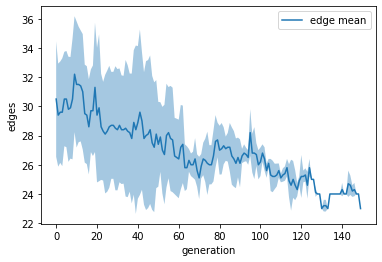
\includegraphics[clip,width=75mm]{edge.png}
    \caption{世代ごとのショートカット数}
    \label{fig:edge}
  \end{center}
\end{figure}

\begin{figure*}[tb]
 \begin{minipage}{0.33\hsize}
 	\begin{center}
 		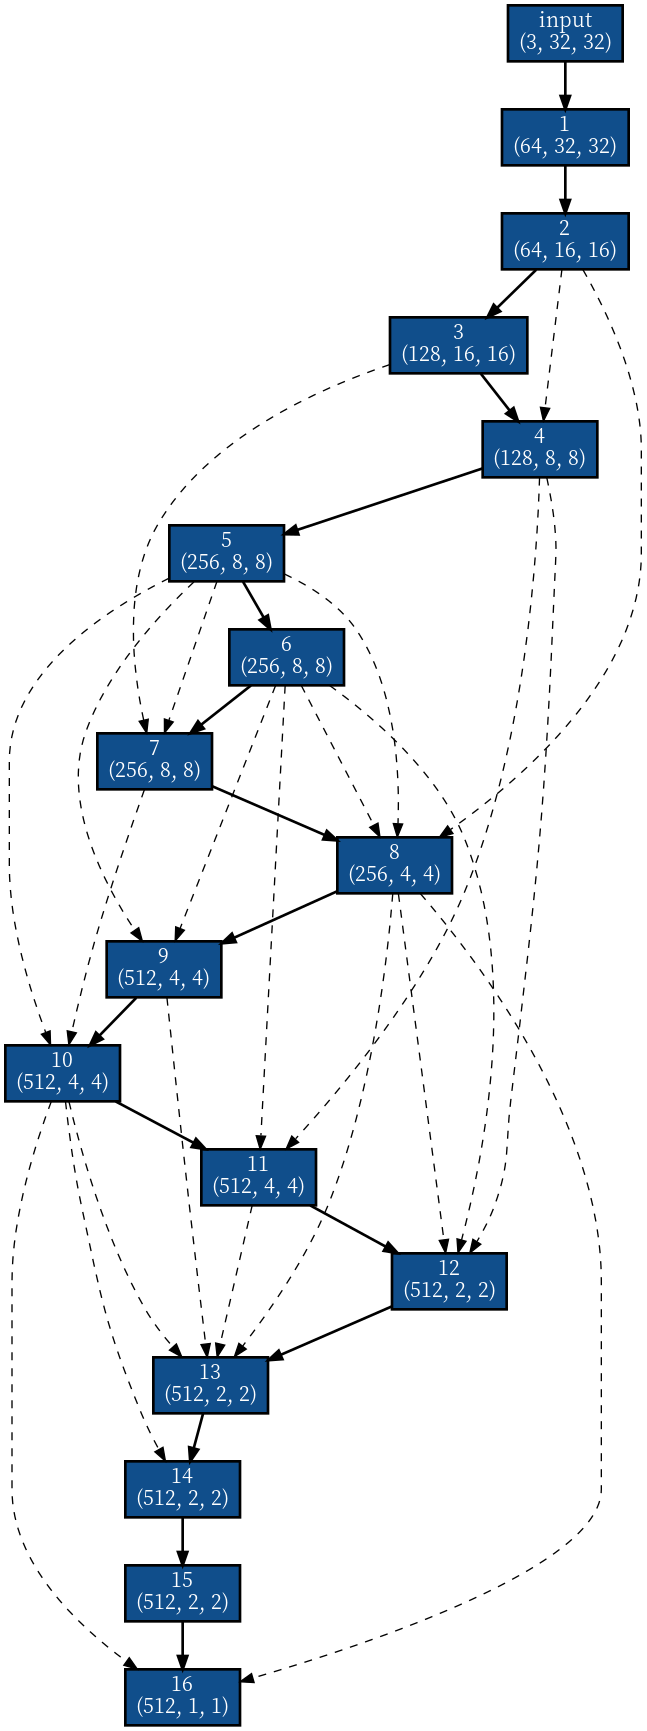
\includegraphics[clip,scale=0.2]{50.png}
 		\caption{50世代目の最良個体}
 		\label{fig:graph50}
 	\end{center}
 \end{minipage}
 \begin{minipage}{0.33\hsize}
 	\begin{center}
 		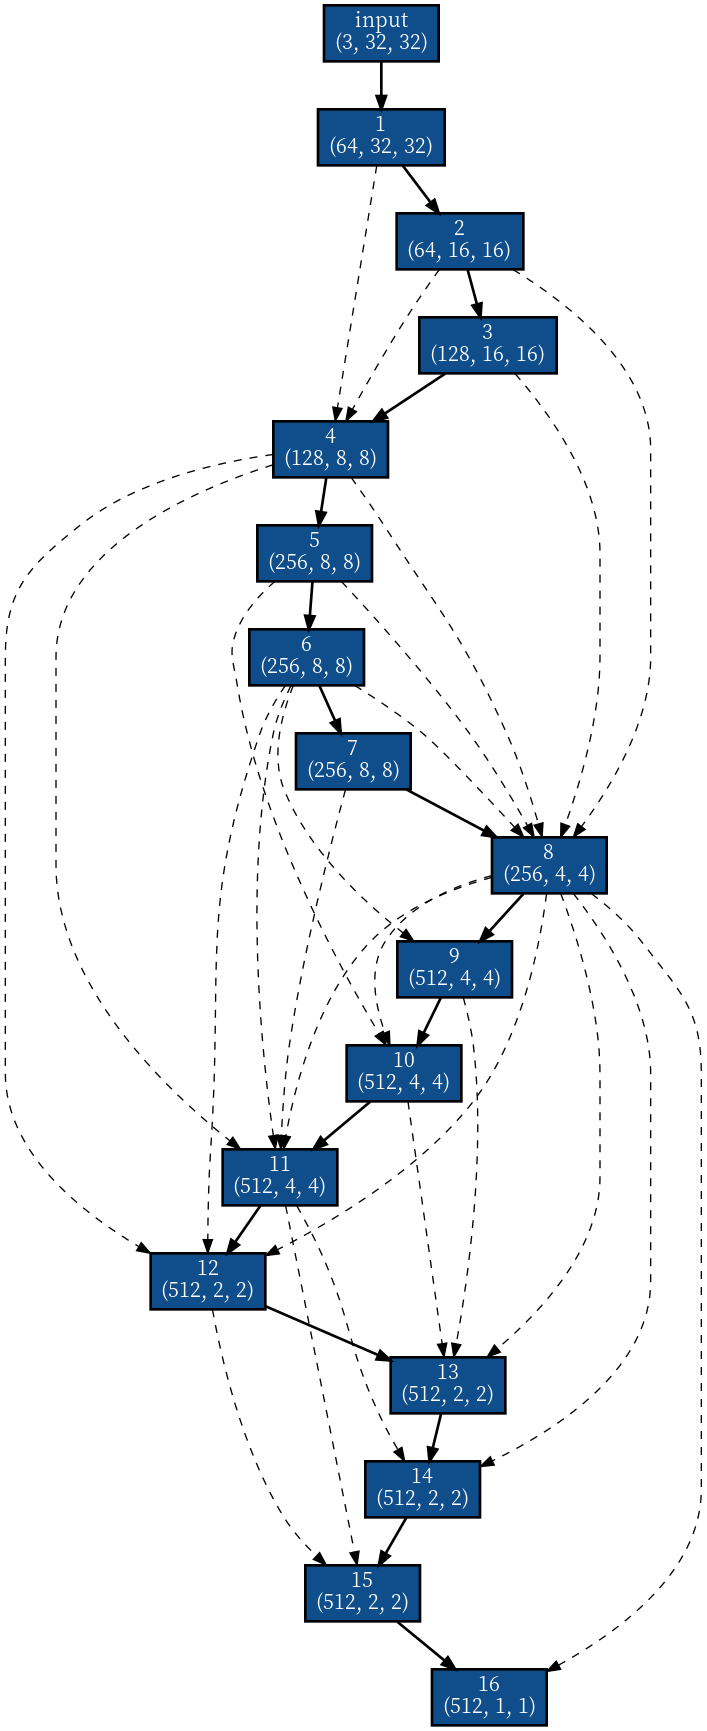
\includegraphics[clip,scale=0.2]{100.png}
 		\caption{100世代目の最良個体}
 		\label{fig:graph100}
 	\end{center}
 \end{minipage}
 \begin{minipage}{0.33\hsize}
 	\begin{center}
 		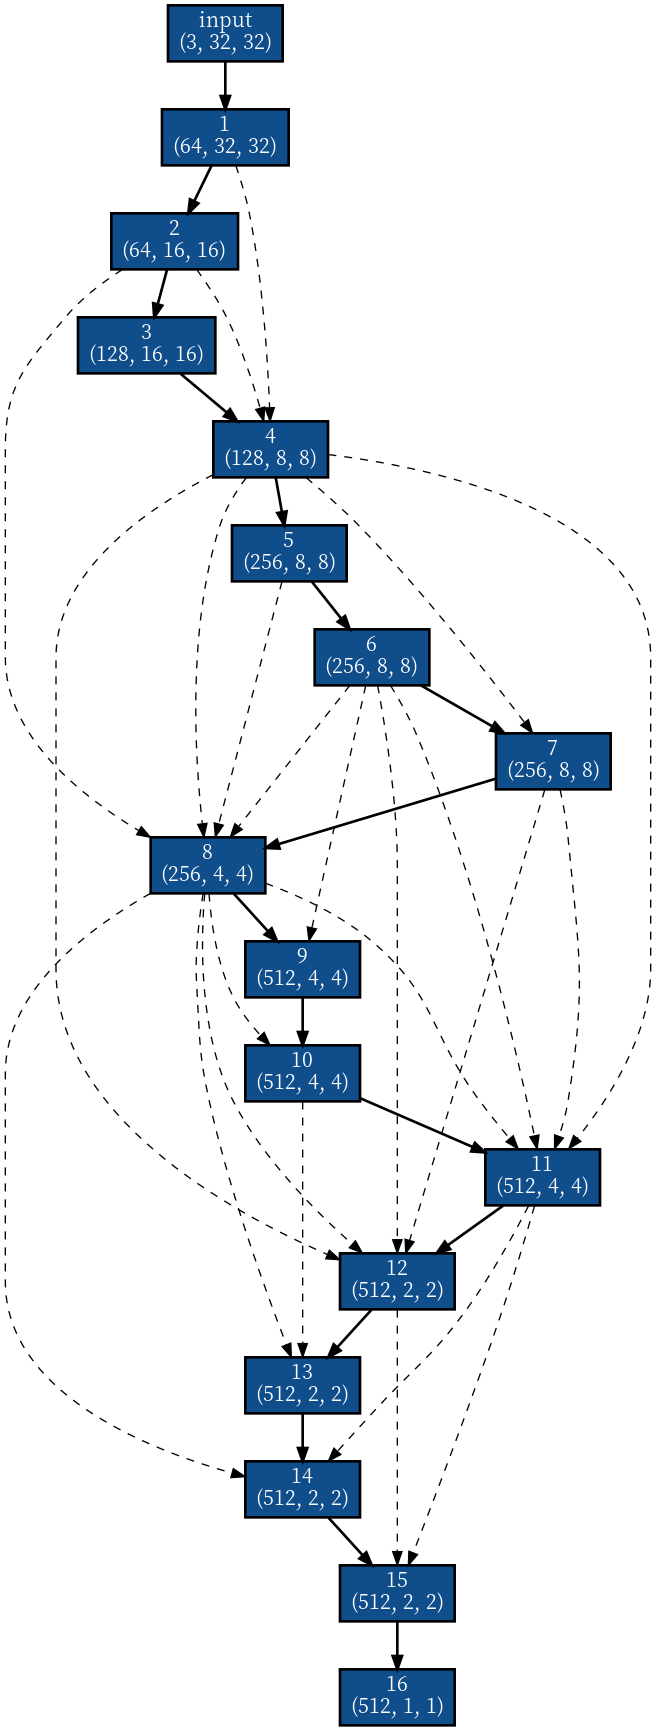
\includegraphics[clip,scale=0.2]{150.png}
 		\caption{150世代目の最良個体}
 		\label{fig:graph150}
 	\end{center}
 \end{minipage}
\end{figure*}

\begin{figure}[tb]
  \begin{center}
    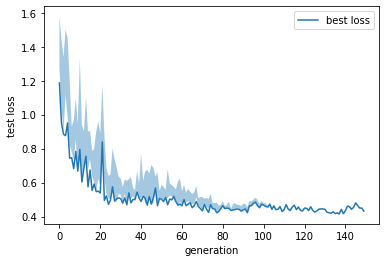
\includegraphics[clip,width=75mm]{loss.png}
    \caption{世代ごとの fitness}
    \label{fig:fit}
  \end{center}
\end{figure}

\begin{figure}[tb]
  \begin{center}
    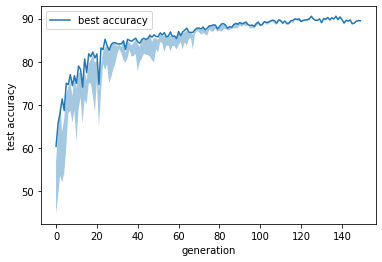
\includegraphics[clip,width=75mm]{acc.png}
    \caption{世代ごとの test accuracy}
    \label{fig:acc}
  \end{center}
\end{figure}


\section{今後の予定}
% なんとなくなんかの勉強をするとかではなく具体的に
\begin{itemize}
  \item 最適な閾値の確認実験
  \item 卒論

\end{itemize}

% 参考文献リスト
\bibliographystyle{unsrt}
\bibliography{ref}
\end{document}
